\chapter{Background}
\label{background}
% Explain relevant concepts needed to understand the experiments and findings:

% Binary Reverse Engineering:
% \begin{itemize}
%     \item Compilers and compiler levels
%     \item Stripping
%     \item Ghidra
% \end{itemize}

% NLP for code:
% \begin{itemize}
% \item Code Summarization
% \item Transformers and CodeT5
% \item Scoring methods
% \end{itemize}

% \newpage
In this chapter, we will cover the required background knowledge to understand this thesis and discuss the relevant works. We will start by covering different aspects of binary reverse engineering. Firstly, compilers and compiler optimization levels will be covered, and then stripping will be explained. Finally, we will discuss the Ghidra toolkit and the relevant modules. The second part of this chapter will feature an explanation of Natural Language Processing methods for code. We will start by explaining the code summarization task, we will then move on to explain transformers and CodeT5. Finally, the BLEU, METEOR and ROUGE evaluation metrics will be explained in detail.
\section{Binary Reverse Engineering}

\subsection{Compilers and Optimization Levels}
Compilers are programs that translate code from one language to another, but generally, and in the context of this thesis, the term is used to refer to programs that translate high-level code, like C, to a lower-level language such as machine code. For our work we focus on the GNU Compiler Collection (GCC)\footnote{gcc: \url{https://gcc.gnu.org/}} and Clang/LLVM (Clang)\footnote{Clang: \url{https://clang.llvm.org/}}.

Compilers frequently feature optimization levels. Generally, the goal of optimizations is the improvement of runtime performance or program size at the expense of compilation time and the ability to debug \cite{ColeOptimizationLevel}. Compilers generally use optimization flags, grouped into optimization levels, where each level uses a different set of optimization flags.

For example, the GCC features 60 optimization flags across 8 different optimization levels, which are denoted by a -O option \cite{ColeOptimizationLevel, gccOptimization}. By default, if GCC is invoked without any optimization options, the program will be compiled with O0. O1, 02 and O3 incrementally apply more optimization to the binary at the expense of a higher compilation time \cite{gccOptimization}. These optimization levels are also found in other compilers such as Clang-LLVM. Other optimization levels, such as Os, which optimises for binary size, are also included in GCC \cite{gccOptimization}.

Optimizations can restructure and transform the program in relation to the source code, by changing the control flow or the data of the program \cite{optimizationObfuscation}. This obfuscation can complicate the reverse engineering process by reducing the accuracy of Ghidra \cite{optimizationObfuscation}.  

\subsection{Stripping}
Aside from compiling with higher optimization levels, binaries can also be stripped to obfuscate the underlying code and to resist analysis\cite{StochFuzz}. Binaries which have not been stripped still contain a lot of debugging information, which can be used during development. This debug information, like function names, self-defined types etc., can be used to analyse and reverse engineer the binary. Commercial Off-the-Shelf (COTS) software is often stripped to reduce the memory and storage footprint of binary, and to resist analysis to protect the intellectual property of the creator. Many vulnerable and malicious binaries are, unfortunately, also stripped to resist security analysis and hide their faults\cite{Debin}.

Unix and Unix-like operating systems include a strip utility. The strip utility removes any operands that are not necessary for the execution of the binary while ensuring that the execution of the binary remains unchanged, the exact implementation and scope of the utility is left to the implementation\footnote{strip: \url{https://pubs.opengroup.org/onlinepubs/007908799/xcu/strip.html}}. 

The strip utility as implemented in GNU/Linux removes the symbol table from the binary. The symbol table contains the symbol location, type and name. The symbol table can be dumped for a given binary by using the nm command \ref{fig:nm}, which is included in Unix and Unix-like operating systems \footnote{nm: \url{https://pubs.opengroup.org/onlinepubs/9699919799/utilities/nm.html}}. 

\label{fig:nm}
\begin{figure}[!h]
  \centering
\begin{lstlisting}
                 U malloc
                 U memcpy
                 U memset
0000000000000060 r minus_b1.3052
0000000000000040 r minus_b2.3053
0000000000005680 t nonce_function_rfc6979
00000000000000c1 r one.4283
0000000000000120 r output32.4535
00000000000000e0 r pad.4239
00000000001101e0 r secp256k1_const_lambda
0000000000110240 r secp256k1_const_modinfo_fe
0000000000110200 r secp256k1_const_modinfo_scalar
000000000000c7d0 T secp256k1_context_clone
000000000000c690 T secp256k1_context_create
000000000000c920 T secp256k1_context_destroy
0000000000000000 D secp256k1_context_no_precomp
...
\end{lstlisting}
  \caption{Sample output of nm command from secp256k1 \protect\footnote{Bitcoin secp256k1: \protect\url{https://github.com/bitcoin-core/secp256k1}} ECDSA library}
\end{figure}
% FIX THIS, footnote doesnt work

Like higher optimization levels, the use of stripping can greatly complicate the efforts to reverse engineer a binary, as well as reduce the accuracy and effectiveness of reverse engineering tools. 
\newpage
\subsection{Ghidra}
Ghidra is a free and open-source reverse engineering toolkit developed by the US National Security Agency. Ghidra has been in development since the turn of the century and had been in use internally, before being open-sourced in April of the same year.

Ghidra contains many separate analysis modules that allow a reverse engineer to analyse compiled code. The modularity of Ghidra and the inclusion of a scripting engine allow users to add custom modules and scripts. We will specifically focus on the tools used in the process that was used to transform binaries into readable code (see \ref{fig:ghidra}).

\label{fig:ghidra}
\begin{figure}[!h]
  \centering
  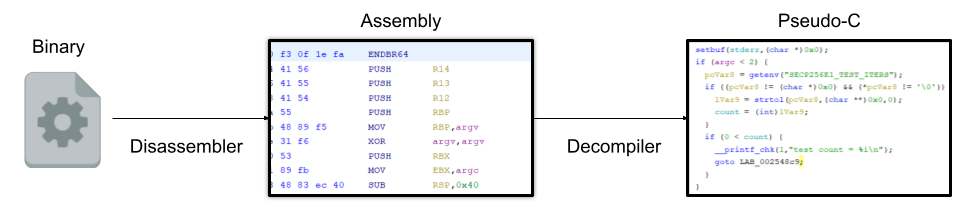
\includegraphics[width=\linewidth]{img/ghidra.png}
  \caption{Transformation of binary to readable code.}
\end{figure}

Ghidra features a disassembler \ref{fig:disassembler}, which will take the binaries and assemble them back into an intermediate representation. In the case of x86-x64 binaries like the binaries this project will focus on, this intermediate representation will be the assembly language. Processors have an associated language that defines the mapping
between user-readable assembly language instructions (e.g. MOV, ADD, etc.) and their corresponding byte values. In order to properly disassemble a binary image for a specific architecture, Ghidra requires a language module for that specific processor. A language module is software that implements language translation. Ghidra has a set of language modules for the most popular processor languages(such as x86-64, ARM, MIPS ..). Besides these architectures which are supporte out-of-the-box, developers have also been extending Ghidra's support with custom processor architectures. For example, there exists a language module for the Allegrex CPU featured in the PlayStationPortable.  \footnote{Ghidra-Allegrex: \url{https://github.com/kotcrab/ghidra-allegrex}}
\label{fig:disassembler}
\begin{figure}[H]
  \centering
  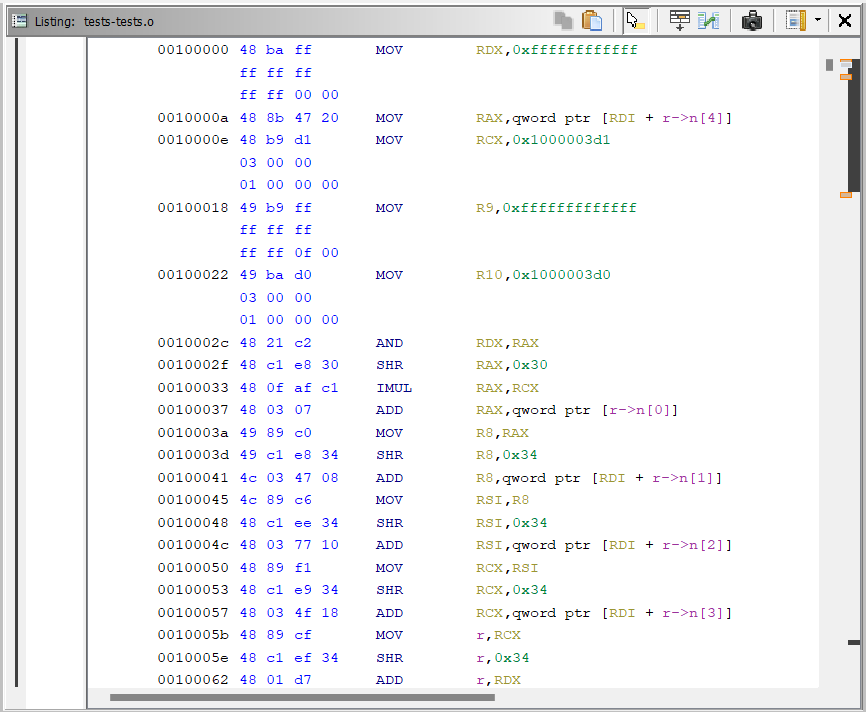
\includegraphics[width=\linewidth]{img/disassembler.png}
  \caption{Ghidra's disassembly window.}
\end{figure}

The decompiler, also featured in Ghidra \ref{fig:decompiler}, is a processor language-agnostic transformation engine that takes the disassembled code and creates a source code representation. The representation is written in pseudo-C, a C-like representation that generally follows the general language conventions of C. The interactive decompiler window allows the user to directly see the correspondence between the pseudo-C and assembly representations. The user can also make changes to the decompiled code, such as changing automatically generated variable names and types and adding comments. 

\label{fig:decompiler}
\begin{figure}[H]
  \centering
  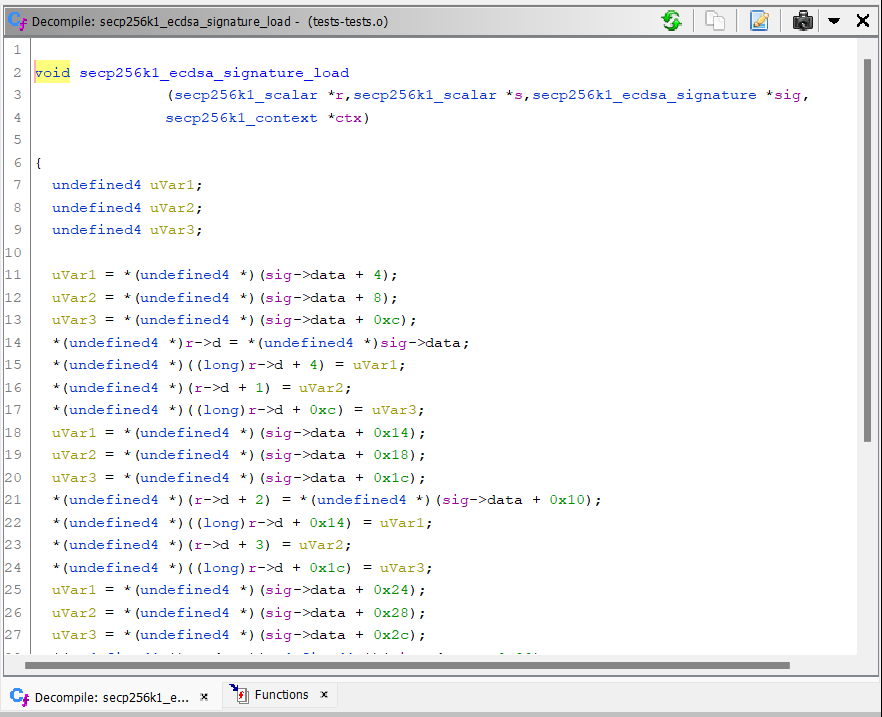
\includegraphics[width=\linewidth]{img/decompiler.png}
  \caption{Ghidra's decompiler window showing a snippet of decompiled function from the secp256k1 ECDSA library}
\end{figure}

\newpage
\section{NLP for Code}

\subsection{Code Summarization}
Code summarization (also referred to as Source code summarization) is the task of writing short descriptions from source code, usually a single sentence summary of the source code. The main use is for software documentation, like the one-sentence JavaDoc description used in Java \cite{leclair_recommendations}. This documentation is important for program comprehension and for maintenance. But the process of writing and maintaining these descriptions is a labour-intensive and time-consuming task, which is where the need to automate that process arises. Code summarization is an extremely active and popular research problem in the field of Software Engineering \cite{leclair_recommendations}.

While code summarization can be applied to any particular piece of code, the problem is usually posed as the generation of a description on the function or method level. A major limitation of these methods is that the model is not provided with any background knowledge. 

A twist on the code summarization task is proposed by \citeauthor{ExtremeSummarization}. Extreme summarization is defined similarly to the code summarization task, but instead of an entire sentence, the model is tasked with summarizing the function in the form of a single descriptive function name.

\subsection{Transformers and CodeT5}
In this thesis, the CodeT5 model, which is based on Transformers, is extensively used. This section provides a quick overview of the Transformer architecture and the CodeT5 model.

\subsubsection{Transformers}
The current state-of-the-art NLP models for programming languages such as CodeT5 \cite{CodeT5}, CodeBERT \cite{CodeBERT} and CodeX \cite{CodeX} are all based on the Transformer architecture \cite{Transformers}.

Transformers were originally proposed by \citeauthor{Transformers} as a novel sequence-to-sequence (seq2seq) architecture. Unlike the recurrent neural networks (RNN), the Long Short-Term Memory (LSTM) variant of RNNs and convolutional neural networks (CNN), Transformers only use a mechanism called self-attention to capture dependencies between the input and output. 

\label{fig:transformers}
\begin{figure}[H]
  \centering
  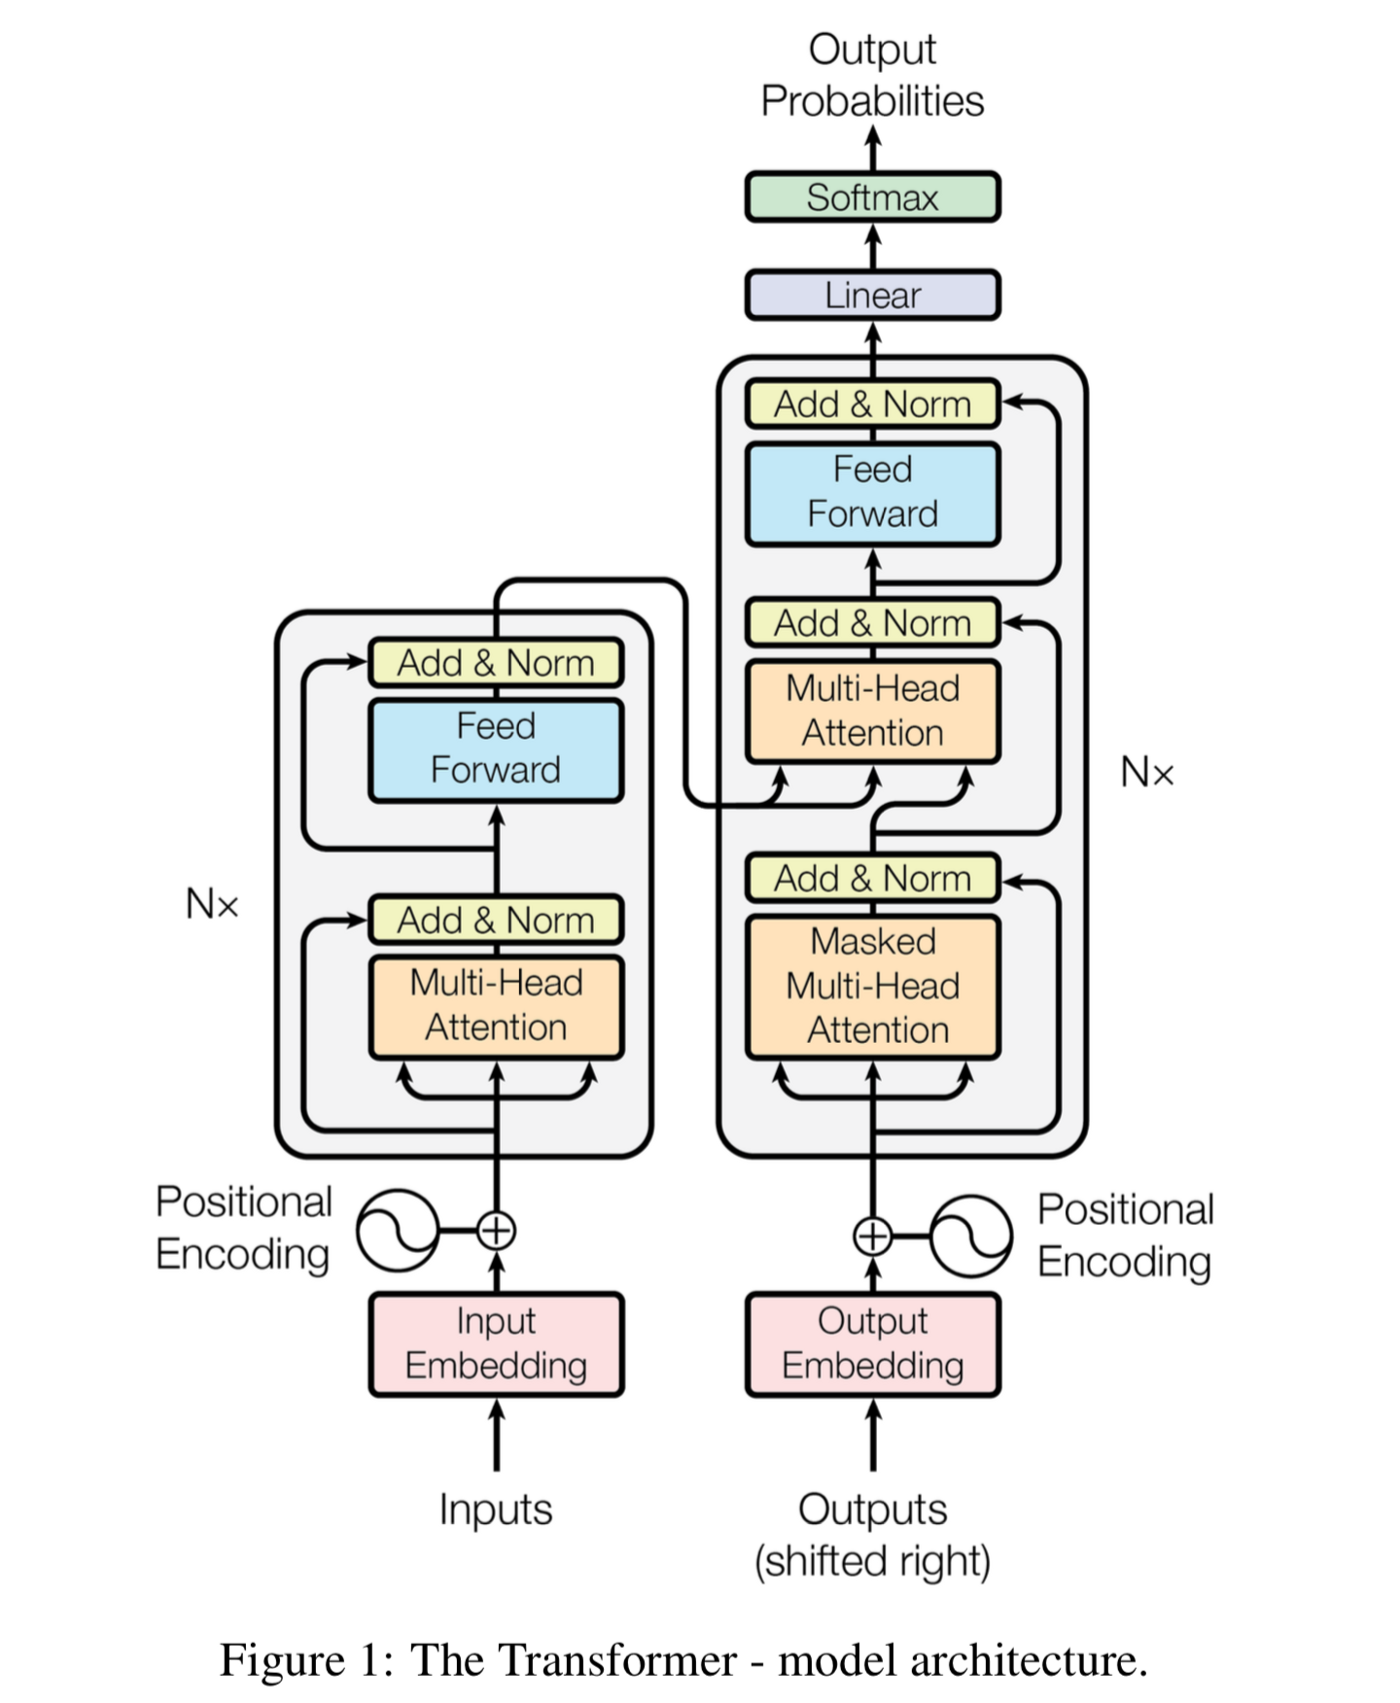
\includegraphics[width=\linewidth]{img/transformer.png}
  \caption{Model overview of Transformer \cite{Transformers}}
\end{figure}

Transformers use an encoder-decoder architecture, where the encoder maps a sequence of input representations \(x = (x_1,x_2 ... x_n)\) to a continuous intermediate representation \(z = (z_1,z_2 ... z_n)\). From this intermediate representation the decoder creates an output \(y = (y_1,y_2 ... y_m)\).

The encoder is comprised of N layers. The input tokens are transformed into an embedding, to every embedded token a positional encoding is added. This positional encoding adds information about the position of every token in the sequence. RNNs receive an \(O(n)\) time penalty for sequential operations on sequences of length \(n\), while sequential operations in Transformers are \(O(1)\) in respect to the length \(n\) of the sequence.

The input is then processed by the self-attention function, which maps a query, and a set of key-value pairs to an output \(Attention(Q,(K,V))\). Intuitively, the query vector \(q\) can be described as the input token, and the mapping finds the most similar key vector \(k\) and outputs the value. This is done by taking the dot product of \(q\) and \(k\), normalizing by dividing by the dimension \(k\) and taking the softmax function. This normalization is important to limit the dot-product values to ensure that the softmax function still retains a good gradient flow. The resulting value \(softmax(\frac{QK^T}{\sqrt{d_k}})\) is maximum when the vectors \(q\) and \(k\) are most similar. Finally this can be multiplied with the value \(v\) to get the value paired with the most similar value \[Attention(Q,(K,V)) = softmax(\frac{QK^T}{\sqrt{d_k}}V)\]
This attention function is applied h times and concatted, and is called the Multi-Head attention layer, where in every attention head different learned weight matrices \(W_i\) are also applied. 
\[MultiHead(Q,K,V) = Concat(head_1, head_2 ... head_h) W^O\]
\[ head_i = Attention(QW^Q_i,KW^K_i,VW^V_i)\] This output is then fed into a Feed-Forward Neural Network and normalized. This single encoder layer, can be stacked N times. This entire process can be parallelized to pass the entire input sequence at once through the encoder. 

The decoder is similarly structured to the encoder. Firstly the target sequence is shifted to the right, such that the model has to predict the next target token. The target sequence is also embedded and the positional encoding is added. The first Multi-Head attention block has masking applied, such that the attention of tokens further in the target sequence is not taken into account while predicting the attention of the current token. Recall that, during training, the model can use the entire input sequence, but only the previous target sequences to predict a token. The mask is a simple upper-triangular matrix, where the upper triangle is set to \(-\infty\) and the lower triangle to \(0\), such that: \[Attention(Q,(K,V)) = softmax(mask + \frac{QK^T}{\sqrt{d_k}}V)\]
This ensures that, during training, the self-attention blocks can still be computed in parallel, without having to resort to sequentially sampling the target.
The next attention block in the decoder implements cross-attention, where the key and value \(K, V\) vectors are fed in from the encoder, and the query \(Q\) vectors are fed in from the previous decoder block. This allows every token in the decoder to attend to all tokens in the encoder, which is important to allow the output to condition to the input. Similarly to the encoder, the final block of the decoder is a feed-forward neural network. The decoder is also stacked N times, and the output of these layers is fed into a Linear Feed Forward Neural Network, which transforms the embedding into a vector of probabilities for every token in the vocabulary of the model. Then the Softmax is applied to the output of the network and the highest probability token is selected as the output. During training, the model is tuned to maximise the probability of predicting the correct output token given the input to the encoder.

Transformers offer a variety of advantages over RNNs and CNNs:
\begin{description}
    \item[Parallelizability] Transformers can process the entire input sequence in parallel. This allows them to leverage the high number of processing cores in conventional GPU architectures, which makes them much faster to train and deploy.
    \item[Long Memory] The Self-Attention paradigm allows the model to establish and remember dependencies along the entire length of the input sequence, the length of the input does not restrict the dependencies. Furthermore, because the model is not recursive in nature and the self-attention vector is calculated for the entire input, the memory gradient does not vanish as with CNNs.
    \item[Interpretability and Explainability] Unlike the black-box nature of RNNs and CNNs, the Self-Attention gradient of the multi-head attention layers can be visualized to show the dependencies between different tokens of the input and output.
\end{description}

\subsubsection{Transfer Learning}
Pre-trained Transformers-based language models, such as RoBERTa, CodeBERT \cite{CodeBERT} and CodeT5 \cite{CodeT5} utilize a pre-train and fine-tune paradigm. In this paradigm, the models are first trained in an unsupervised manner on a large unlabeled dataset. In the case of RoBERTa, a Masked Language Modeling (MLM) objective was used, where random tokens are masked out from a swath of text (or code in CodeBERTs case) and the model is tasked to predict said tokens. These pre-trained models can then be fine-tuned to perform a more specialized task, such as summarization. This concept is called transfer learning (TL). 
TL uses the knowledge that is obtained in one task to solve a different task. It allows the creation of general models that are trained once on massive (usually unlabeled) datasets. These general models, which contain general domain knowledge can then be trained for a specific downstream task. In general, this approach is quicker and requires less training data than training a model on the downstream task from scratch\cite{BERT}.

\subsubsection{CodeT5}
CodeT5 is a SOTA pre-trained programming language model built on the T5 (Text-to-text Transfer Transformer) architecture proposed by \citeauthor{CodeT5} and pre-trained on a mix of unsupervised and supervised tasks. CodeT5 employs an encoder-decoder architecture, other state-of-the-art models only feature an encoder (BERT) or a decoder (GPT).
In contrast to other models, CodeT5 is trained using both unimodal (PL only) and bimodal (NL to PL) tasks in six programming languages. This bimodal training allows CodeT5 to have strong performance in both uni-modal (PL-to-PL) tasks such as code translation and code refinement, as well as cross-modal tasks such as code summarization and code generation (PL-to-NL).

\subsection{Scoring Methods}
To evaluate the quality of the source code summaries an evaluation metric is required, which quantifies the quality of a produced candidate summary compared to a reference. The simplest metric is an exact match score, where the score is 1 if the candidate matches the reference exactly. This metric does not reflect the actual quality of the produced summary.

\subsubsection{BLEU}
The most widely used metric in the Code Summarization task is Bilingual Evaluation Understudy Score (BLEU) \cite{evaluationSummarization}. BLEU was originally proposed as a technique to evaluate the machine translations against a set of human translations. In the code-summarization domain, the automatically generated summaries are compared against a programmer defined summary. 
BLEU produces a percentage number between 0 and 100, which defines the similarity between a candidate and a set of reference sentences. BLEU-N calculates the cumulative N-gram precision scores, the number of matching N-grams divided by the total number of N-grams in the candidate sentence. The unigrams (1-grams) account for the adequacy of the candidate while the longer N-grams account for the fluency. 
Two problems arise, firstly the score can be artificially inflated by simply repeating the same matching N-gram multiple times in the candidate \ref{tab:BLEUIssues}. Secondly, the score can also be inflated by creating a very short candidate such that the denominator is very small \ref{tab:BLEUIssues}.

\label{tab:BLEUIssues}
\begin{table}[H]
\begin{tabular}{l|lllllll|l}
\rowcolor[HTML]{C0C0C0} 
Reference & Calculate & the & Secp256k1 & private & key & given & generator & Precision \\ \hline
Repeating & the       & the & the       & the     & the & the   &           & 6/6 = 1   \\
Short     & Calculate &     &           &         &     &       &           & 1/1 = 1  
\end{tabular}
\caption{An example of a repeating and short candidate, and the resulting 1-gram precision.}
\end{table}

To counteract these two issues, BLEU firstly clips the n-grams in the numerator, such that each match is only counted once. Secondly, a Brevity Penalty (BP) is applied such that a short candidate is penalized. Recall that long candidates are already inherently penalized by the precision metric. Let \(c\) be the length of the candidate and \(r\) be the length of the reference, BP is then defined as:

\begin{equation}
  BP=\begin{cases}
    1, & \text{if $c<r$}.\\
    e^{(1 - r/c)}, & \text{otherwise}.
  \end{cases}
\end{equation}
The geometric mean of each of the clipped n-gram precision scores \(p_n\) is taken:
\[ \text{BLEU-N} = BP \cdot exp(\sum_{n=1}^{N} w_n log p_n ) \]
Where \(w_n\) is a uniform weight \(w_n = 1/N\).

While \(N\) could be any number, BLEU-4 is the most commonly used variant. Since code summaries are generally quite short and the BLEU score was originally designed for use in longer corpora of text it can occur that there are no matching 4-grams between a candidate and reference summary\cite{evaluationSummarization}. The geometric mean will then result in 0, and the BLEU score will also be 0. To solve this, smoothing is applied. There exist a variety of smoothing methods, which all add a factor to the numerator and denominator of \(p_n\) \cite{evaluationSummarization}.

\label{tab:BLEUScale}
\begin{table}[H]
\begin{tabular}{l|l}
\hline
\rowcolor[HTML]{E8EAED} 
\multicolumn{1}{|l|}{\cellcolor[HTML]{E8EAED}{\color[HTML]{202124} \textbf{BLEU Score}}} & \multicolumn{1}{l|}{\cellcolor[HTML]{E8EAED}{\color[HTML]{202124} Interpretation}} \\ \hline
\rowcolor[HTML]{FFFFFF} 
{\color[HTML]{202124} \textless 10}                                                      & {\color[HTML]{202124} Almost useless}                                              \\
\rowcolor[HTML]{FFFFFF} 
{\color[HTML]{202124} 10 - 19}                                                           & {\color[HTML]{202124} Hard to get the gist}                                        \\
\rowcolor[HTML]{FFFFFF} 
{\color[HTML]{202124} 20 - 29}                                                           & {\color[HTML]{202124} The gist is clear, but has significant grammatical errors}   \\
\rowcolor[HTML]{FFFFFF} 
{\color[HTML]{202124} 30 - 40}                                                           & {\color[HTML]{202124} Understandable to good translations}                         \\
\rowcolor[HTML]{FFFFFF} 
{\color[HTML]{202124} 40 - 50}                                                           & {\color[HTML]{202124} High quality translations}                                   \\
\rowcolor[HTML]{FFFFFF} 
{\color[HTML]{202124} 50 - 60}                                                           & {\color[HTML]{202124} Very high quality, adequate, and fluent translations}        \\
\rowcolor[HTML]{FFFFFF} 
{\color[HTML]{202124} \textgreater 60}                                                   & {\color[HTML]{202124} Quality often better than human}
\end{tabular}
\caption{Interpretation of BLEU scores \cite{evaluationSummarization}}
\end{table}

A major weakness of the BLEU metric is the fact that it does not consider the meaning of the reference and candidate texts, synonyms and syntactically different texts have a low score despite their adequacy. For example, a reference of "Calculate the Secp256k1 private key given the generator" and a candidate of "Secp256k1 secret key calculation from G" will score very lowly, despite the fact that they both convey the same information. 

\subsubsection{METEOR}
METEOR (Metric for Evaluation for Translation with Explicit Ordering) \cite{Meteor} is also a metric proposed to assess a machine-generated translation against multiple human-generated references. Unlike BLEU which is a precision-based metric, METEOR is more recall-focused. METEOR has a higher correlation with human judgement than BLEU \cite{recommend_summarization}, it uses wordlists and stemming to also take synonyms into account. On the flip side, the stemming and synonyms are language-dependent and somewhat more expensive than BLEU to calculate.

The METEOR score is calculated by first generating an alignment between a candidate and the reference sentence. An alignment is a mapping between each unigram (or word) in the candidate and reference sentences. The unigrams can be matched in 3 ways: Firstly the unigrams can be an \textit{exact} match. The unigrams can also be matched on the \textit{stem}, which will match words on their stem. For example the words 'improved' and 'improving' will both be reduced to their stem 'quick' and will then be matched. Finally, words can also be matched if they are synonyms, for instance 'quick' and 'fast'. This is determined using the WordNet database. The alignment which best preserves the word order is selected. 

A fragmentation penalty (p) is also introduced to account for congruity. The minimum number of adjacent matched groups (or chunks) of words in the candidate and reference. The penalty \(Pen\) is calculated as a function of the number of chunks \(ch\), the number of matches \(m\) hyperparameters \(\gamma, \beta\).

\begin{equation}
\begin{aligned}
frag = \frac{ch}{m} \\
Pen = \gamma * frag^{\beta}
\end{aligned}
\end{equation}

The selected alignment is then scored using a harmonic mean:

\begin{equation}
  \begin{aligned}
P = \frac{m}{t} \\
R = \frac{m}{r} \\
F_{mean} = \frac{P*R}{\alpha * P * (1 - \alpha) * R} \\
Score = (1 - Pen) * F_{mean}
\end{aligned}
\end{equation}

\subsubsection{ROUGE-L}
ROUGE or Recall-Oriented Understudy for Gisting Evaluation, is a package which includes a number of metrics, the most popular among them is ROUGE-L \cite{Rouge}. As the name implies, it is more recall oriented than BLEU. Unlike BLEU and METEOR, the ROUGE measures were constructed to score automatically generated candidate summaries against one or multiple reference summaries. ROUGE-L is much quicker than METEOR to calculate and is language-independent. 

ROUGE-L simply finds the longest common subsequence (LCS) between the reference and the candidate, note that the words do not need to be consecutive but they have to be in order. The length of the LCS \(lcs\), the length of the reference \(r\), the length of the candidate \(c\), and a large constant \(\beta \rightarrow \infty\) are then used to calculate the score:
\begin{equation}
  \begin{aligned}
P = \frac{lcs}{c} \\
R = \frac{lcs}{r} \\
ROUGE-L= \frac{(1+\beta^2)*R*P}{R+ \beta^2 * P} \\
\end{aligned}
\end{equation}


